% 
% Septiembre 2020
% Author: Mathieu Kessler
% Universidad Politécnica de Cartagena
% https://personas.upct.es/perfil/mathieu.kessler
% 
% 
\documentclass[9pt]{beamer}
\definecolor{links}{HTML}{2A1B81}
\hypersetup{colorlinks,linkcolor=,urlcolor=links}
\usepackage[spanish]{babel}
\usepackage{colortbl}
\usepackage{graphicx}
\usepackage{amsmath,amssymb}
\usepackage{comma}
\usepackage{fancybox,color}
\usepackage[utf8]{inputenc}
\graphicspath{{../figures/}}
\setbeamertemplate{navigation symbols}{}
% \usepackage[colorlinks=true]{hyperref}
\usepackage{xcolor}
\definecolor{mycodecolor}{rgb}{0.65,0.25,0.1}

\usepackage{listings}
\newcommand{\inlinecode}[2][Python]{\lstinline[language=#1, basicstyle=\color{mycodecolor}]{#2}}
\usepackage{beamerthemeshadow}
\usepackage{xmpmulti}
\usepackage{mathtools}
\DeclarePairedDelimiter\abs{\lvert}{\rvert}%
\usepackage{tabularx}
\renewcommand\tabularxcolumn[1]{b{#1}}
\newcommand{\field}[1]{\mathbb{#1}}
\newcommand{\E}{\field{E}}
\newcommand{\R}{\field{R}}
\newcommand{\N}{\field{N}}
\newcommand{\Z}{\field{Z}}
\newcommand{\Q}{\field{Q}}
\newcommand{\EE}{\field{E}}
\newcommand{\FF}{\field{F}}
\newcommand{\GG}{\field{G}}
\renewcommand{\L}{\field{L}}
\renewcommand{\P}{\field{P}}
\newcommand{\LL}{{\mathfrak L}}


\begin{document}
\lstset{language=Python}
\title{Preparando vuestro entorno Python para la asignatura (I):\\
  Instalar Python usando Anaconda.}

\author[Mathieu Kessler]{Mathieu Kessler}
\institute[]{Departamento de Matemática Aplicada y Estadística \\ Universidad Politécnica de Cartagena}
%% \date{\textcolor{blue}{Granada, 5 de abril de 2019}}
\titlegraphic{
\includegraphics[width=6cm]{python_anaconda}}

\begin{frame}
  \titlepage
\end{frame}

\begin{frame}
  \frametitle{Instalar Python usando Anaconda}
  Existen diferentes maneras de instalar Python. En este curso,
  usaremos la distribución Anaconda, que facilita la gestión de librerías.\\
  Dos opciones son posibles:
  \begin{enumerate}
  \item \textbf{El entorno completo}. Usa la distribución de Anaconda
    más completa. Es la mejor elección si tenéis 3GB de espacio libre
    en vuestro disco y os gusta la idea de tener 250 librerías
    científicas instaladas por defecto. El repositorio de Anaconda
    facilita la instalación de librerías adicionales.
    \begin{center}
      
\includegraphics[width=2cm]{anaconda_logo}
    \end{center}

  \item \textbf{El entorno ``Miniconda'' }. Usa la distribución Miniconda
    distribution, que ocupa poco espacio (300 MB). Sobre esta
    distribución minimalista, habrá que instalar manualmente las
    librerías requeridas (numpy, scipy,
    matplotlib, pandas)
    \begin{center}
      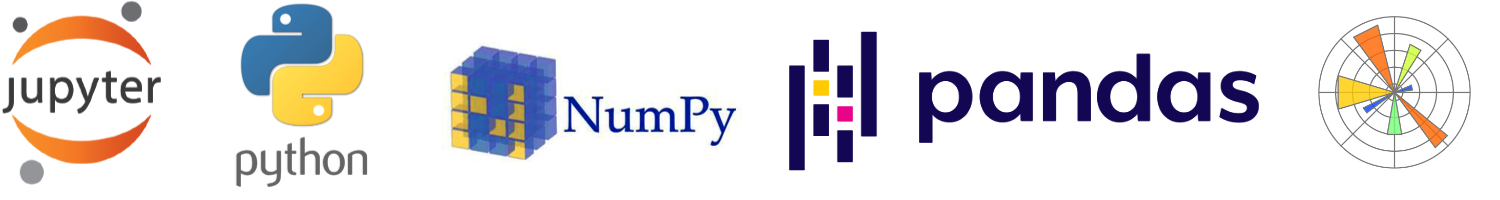
\includegraphics[width=8cm]{jupyter_python_numpy_pandas}
    \end{center}

  \end{enumerate}
\end{frame}
\begin{frame}
  \frametitle{Comparando las dos opciones}
  \begin{block}{Notas}
    \begin{itemize}
    \item       \begin{tabular}[h]{b{5cm}m{3cm}}
                  \parbox[t]{5cm}{ Para este asignatura, hasta cierto
                  punto, la opción 1 es innecesaria (``a sledgehammer to
                  crack a nut.'')}&
                                 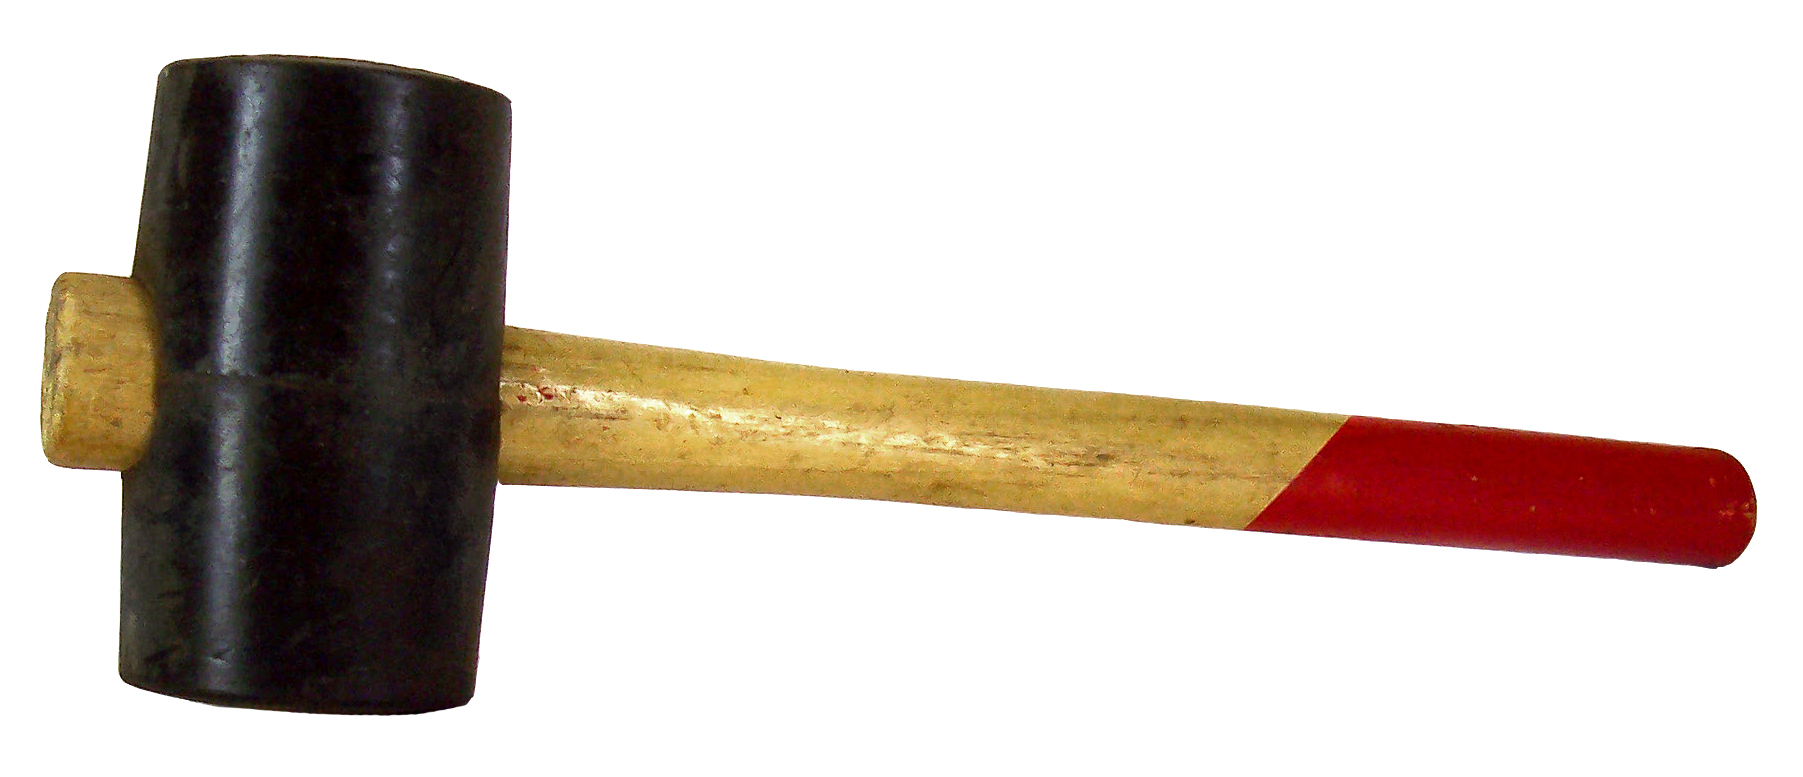
\includegraphics[width=3cm]{sledgehammer-nut.png}
                                 
                \end{tabular}\\
                Pero, facilita la gestión de las librerías y es una
                buena opción si vais a usar Python para proyectos más complejos.
                \pause
              \item Oiréis hablar de Python 3 y Python 2. En este
                curso, usaremos Python 3.\\
                \begin{center}
                  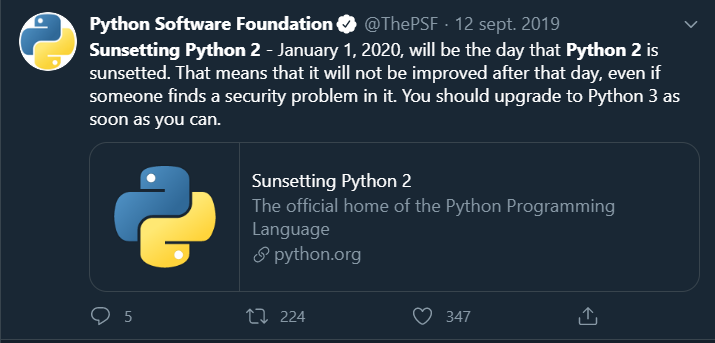
\includegraphics[width=5cm]{sunsetting_python_2.png}
                  \href{https://www.python.org/doc/sunset-python-2/}{https://www.python.org/doc/sunset-python-2/}
                \end{center}

              \end{itemize}
            \end{block}

          \end{frame}

        % \begin{frame}
          %   \frametitle{Option 2: installation of the ``Miniconda'' environment}
          %   \Ovalbox{  The following only applies if you have chosen to install the
          %   ``bare'' environment.}\\ \medskip
          %   The simplest way to install Python 3 on Windows is to use the
          %   Microsoft Store.\includegraphics[width=0.5cm]{microsoft_store.png}
          %   \begin{center}
          %     \includegraphics[width=10cm]{python_microsoft_store.png}
          %   \end{center}
          %   Check that the publisher is the Python Software Foundation.\\
          %   \begin{block}{}
          %     \textit{\scriptsize A full installer is also available from the Python
          %     Software Foundation, it
          %     includes all components and is more complete than the Microsoft Store
          %     installer. More information here: \href{https://docs.python.org/3/using/windows.html}{https://docs.python.org/3/using/windows.html}
          %   }
          %   \end{block}
          % \end{frame}
          % \begin{frame}
          %   \frametitle{Option 2: installation of the ``bare'' environment}

          %   To check that Python was properly installed on your system, type {\tt
          %   python} in a {\tt cmd} window shell:
          %   \begin{center}
          %     \includegraphics[width=10cm]{python_cmd}
          %   \end{center}

          %   \begin{block}{}
          %     \textit{ To exit the python shell, type {\tt quit()} at the
          %     prompt}
          %   \end{block}
          
          % \end{frame}
          % \begin{frame}
          %   \frametitle{Option 2: installation of the ``bare'' environment}
          %   {\huge Installing the required packages for the course} 
          %   \begin{block}{Packages' installation and management in Python}
          %     The package manager in Python is {\tt pip}, which, in particular,
          %     retrieves packages from {\tt \tt PyPI} \href{https://pypi.org/}{https://pypi.org/}, the Python Package Index, a huge
          %     repository of software developed and shared by the Python community.
          %   \end{block}
          %   We will install the following packages for the course:\smallskip

          %   \begin{tabular}[h]{ll}
                %                 $\bullet$ {\tt numpy}&\onslide<2->{A package for scientific
                                                         %                                                          computing. \href{https://numpy.org/}{https://numpy.org/}}\\[0.2cm]

                                                         %                          %                                                          \verb{@numpy_team}}\\
                %                 $\bullet$ {\tt scipy} & \onslide<3->{\parbox{8.5cm}{Numerical routines: integration, interpolation,
                                                          %                                                           optimization, linear algebra, and statistics
                                                          %                                                           \href{https://www.scipy.org}{https://www.scipy.org}}}\\[0.3cm]
          
                %                 $\bullet$ {\tt matplotlib} & \onslide<4->{\parbox{8.5cm}{Library for
                                                               %                                                                creating static, animated, and
                                                               %                                                                interactive visualizations
                                                               %                                                                \href{https://matplotlib.org/}{https://matplotlib.org/}}}\\[0.3cm]
          
                %                 $\bullet$ {\tt pandas} & \onslide<5->{\parbox{8.5cm}{Data analysis and
                                                           %                                                            manipulation \href{https://pandas.pydata.org/}{https://pandas.pydata.org/}                           
                                                           %                                                            }}\\[.2cm]
          
                %                 $\bullet$ {\tt jupyter} &\onslide<6->{\parbox{8.5cm}{
                                                            %                                                             Provides an interactive development
                                                            %                                                             environment for computing through
                                                            %                                                             notebooks for a variety of programming languages.\href{}{}
                                                            %                                                             }}
                                                            %               \end{tabular}
                                                            %                                                             \end{frame}
                                                            %                                                             \begin{frame}
                                                            %                                                             \frametitle{Option 2: installation of the ``bare'' environment}
                                                            %                                                             \begin{block}{The instruction to install a package from {\tt PyPI}}
                                                            %                                                             To install a package called ``package\_to\_install'', type in the
                                                            %                                                             command shell:\\\smallskip
          
                %                 {\tt python -m pip install --user package\_to\_install }
          
                %                 \end{block}\pause
                %                 We will therefore start by installing {\tt numpy}

                %                 \begin{center}
                %                 \includegraphics[height = 2cm]{pip_install_numpy}
                %                 \end{center}
                %   %                 \begin{center}
                %   %                   \includegraphics[height = 1.5cm]{pip_install_scipy}
                %   %                 \end{center}
                %   %                 \begin{center}
                %   %                   \includegraphics[height = 1.5cm]{pip_install_matplotlib}
                %   %                 \end{center}
                %   %                 \begin{center}
                %   %                   \includegraphics[height = 1.5cm]{pip_install_pandas}
                %   %                 \end{center}
                %   %                 \begin{center}
                %   %                   \includegraphics[height = 1.5cm]{pip_install_jupyter}
                %   %                 \end{center}
                %                 \pause And similarly
                %                 \begin{block}{}
                %                 {\tt python -m pip install --user scipy }\\\smallskip
                %                 {\tt python -m pip install --user matplotlib }\\\smallskip
                %                 {\tt python -m pip install --user pandas }\\\smallskip
                %                 {\tt python -m pip install --user jupyter}
          
                %                 \end{block}
                %                 \end{frame}
          
          \begin{frame}
            \frametitle{Opcion 1: usando la distribución Anaconda}
            \begin{tabularx}{\linewidth}{XX}
              
\includegraphics[width=0.4\textwidth]{anaconda_logo_big}
              &
              \parbox{0.5\textwidth}{    La distribución Anaconda
                (Individual Edition) es open-source y está diseñada
                especialmente para  data science y  machine learning. \\
                Viene con más de 250 librerías preinstaladas, lo que
                la convierte en una solución sencilla para trabajar
                con Python en Data Science. Paquetes
                adicionales se pueden descargar desde el repositorio
                de Anaconda}

            \end{tabularx}\bigskip
            \begin{center}
              {\huge \href{https://www.anaconda.com/}{https://www.anaconda.com/}}
            \end{center}\medskip

            El producto es la ``Individual Edition'':\\ \smallskip
            {\huge \href{https://www.anaconda.com/products/individual}{https://www.anaconda.com/products/individual}}
          \end{frame}
        
        \begin{frame}
            \frametitle{Opción 1: usando la distribución Anaconda}
            \begin{block}{Para instalar Anaconda}
              \href{https://www.anaconda.com/products/individual}{Descargad
                el ejecutable de instalación}.
              
            \end{block}
            \pause
            \begin{block}{Notas importante para la instalación}
              \begin{itemize}
              \item Instalad  Anaconda en una carpeta cuyo camino en
                el disco no contiene espacios o caracteres unicode
                (acentos, etc...)
              \item
                No añadáis Anaconda a vuestra variable de entorno
                PATH. Podría interferir con la creación de entornos
                virtuales en Python.             
                
                \begin{center}
                  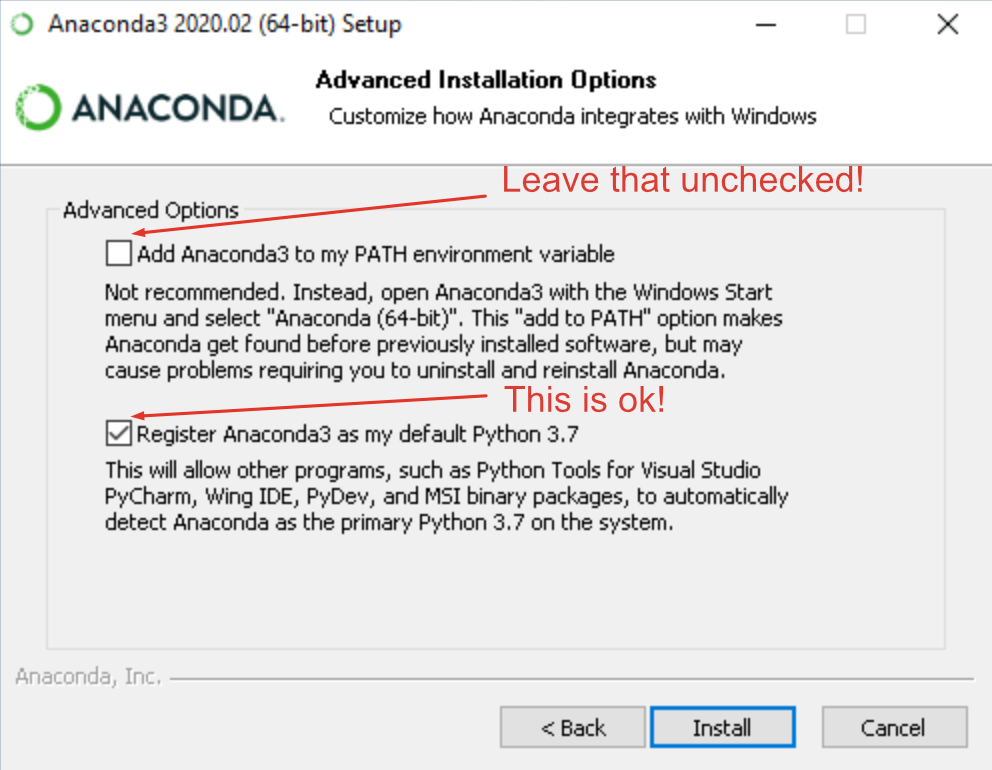
\includegraphics[width=0.4\textwidth]{anaconda_installation_path}
                  
                \end{center}

              \end{itemize}\medskip
              
              
            \end{block}
            Para más información: \href{https://docs.anaconda.com/anaconda/install/}{https://docs.anaconda.com/anaconda/install/}
          \end{frame}

        \begin{frame}
            \frametitle{Opción 1: Usando la distribución Anaconda}
            Podéis comprobar que la instalación se ha realizado correctamente
            lanzando el navegador Anaconda:.
            
            \begin{center}
              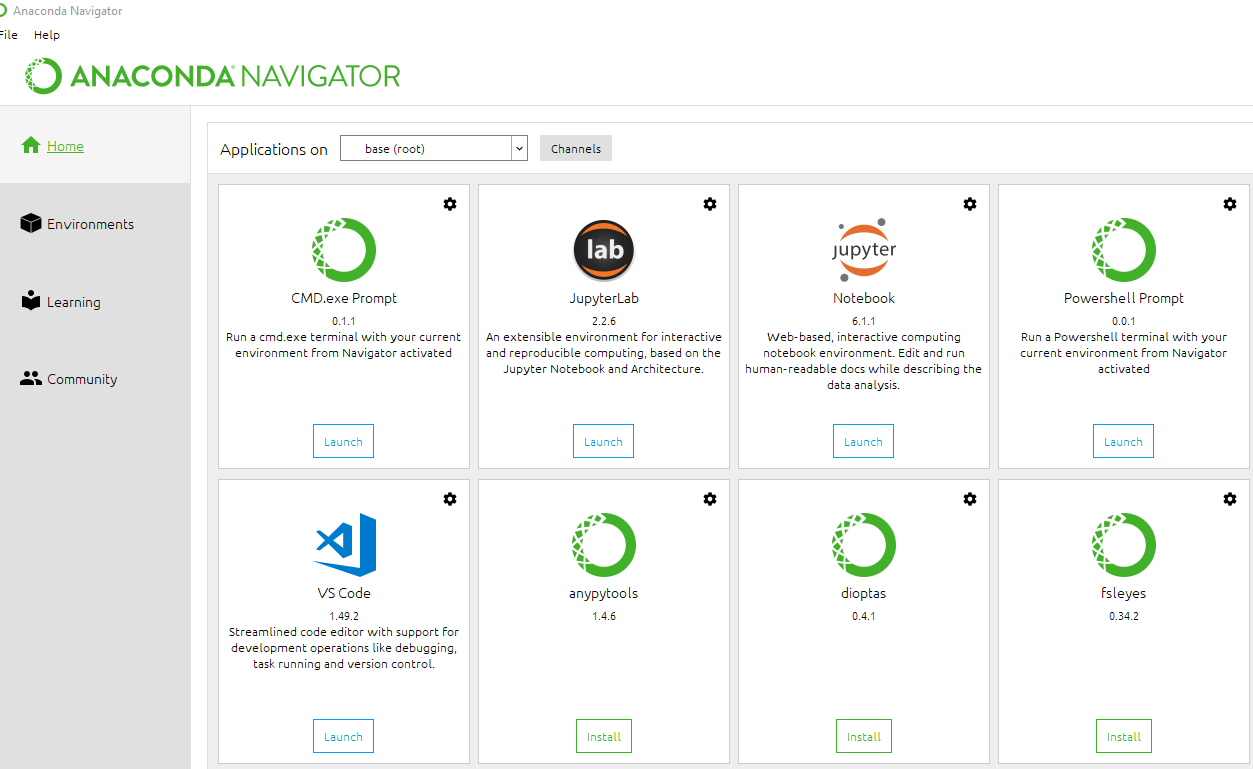
\includegraphics[width=0.4\textwidth]{anaconda_navigator}
              
            \end{center}

            o al lanzar la consola  Anaconda e introducir los comandos
            \inlinecode[bash]{conda list} por ejemplo
            
            \begin{center}
              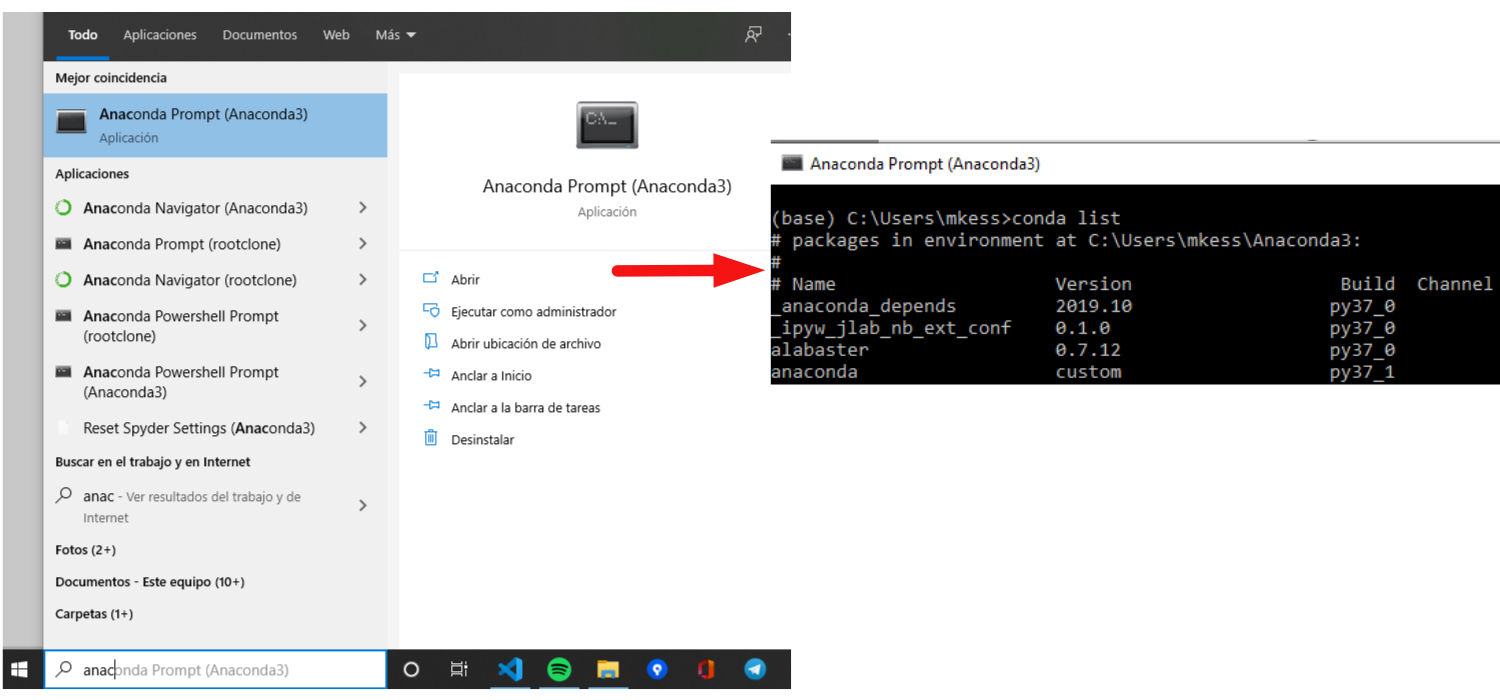
\includegraphics[width=0.9\textwidth]{check_anaconda_prompt}
            \end{center}
            
          \end{frame}
   
        \begin{frame}
            \frametitle{Opción 2: usando la distribución  ``Miniconda''}
            \begin{center}
              {\huge \href{https://docs.conda.io/en/latest/miniconda.html}{https://docs.conda.io/en/latest/miniconda.html}}
            \end{center}\medskip

            \begin{block}{Para instalar Miniconda install Miniconda}
              Descargad el ejecutable de instalación para Python 3, y lanzadlo.
              
            \end{block}
            \pause
            \begin{block}{Notas importantes para la instalación}
             \begin{itemize}
              \item Instalad  Miniconda en una carpeta cuyo camino en
                el disco no contiene espacios o caracteres unicode
                (acentos, etc...)
              \item
                No añadáis Miniconda a vuestra variable de entorno
                PATH. Podría interferir con la creación de entornos
                virtuales en Python.               
                
                \begin{center}
                  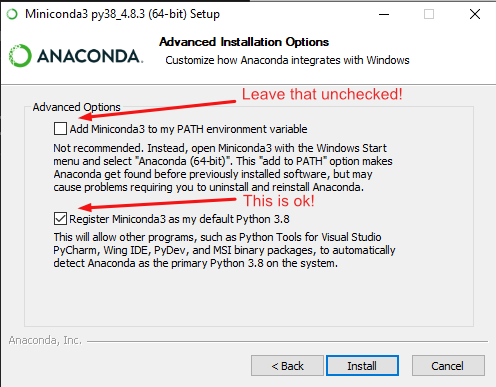
\includegraphics[width=0.6\textwidth]{Miniconda_installation_options}
                  
                \end{center}

              \end{itemize}\medskip
            \end{block}
            Más información en: \href{https://docs.anaconda.com/anaconda/install/}{https://docs.anaconda.com/anaconda/install/}
          \end{frame}
        
        \begin{frame}
            \frametitle{Opción 2: usando la distribución  Miniconda}
            Para comprobar que la instalación se ha realizado
            correctamente, abrid la consola Miniconda (buscad
            ``Miniconda'' en la caja de búsqueda Windows)
            \begin{center}
              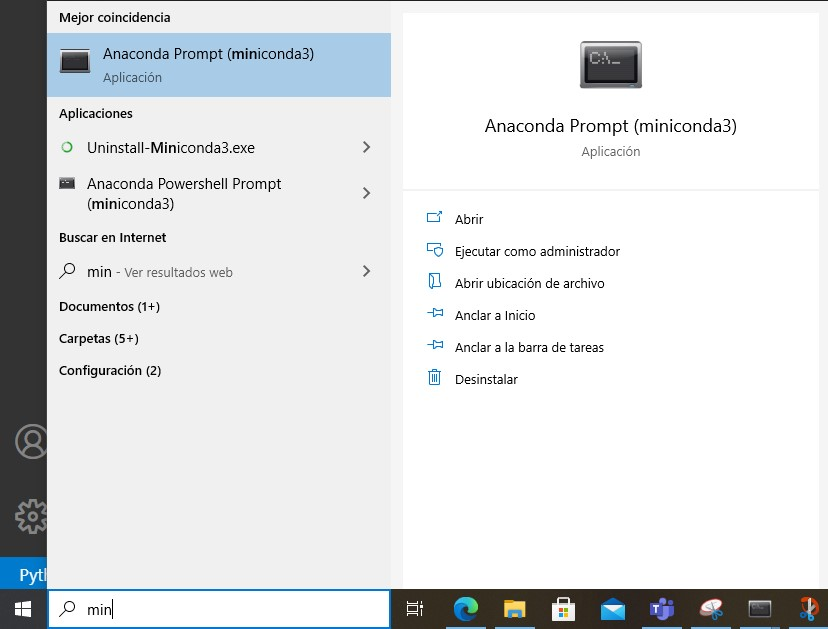
\includegraphics[width=0.4\textwidth]{Miniconda_prompt.jpg}
            \end{center}

            Introducid \inlinecode[bash]{conda list}:
            \begin{center}
              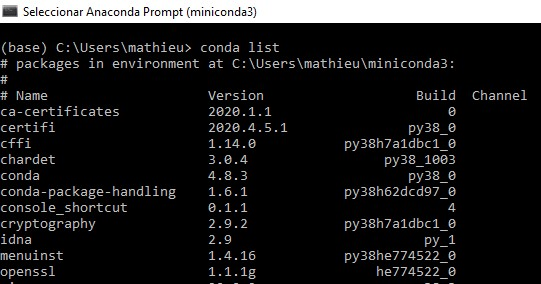
\includegraphics[width=0.8\textwidth]{conda_list}
            \end{center}
            
          \end{frame}


          \begin{frame}
            \frametitle{Cómo interactuar con Python en mi sistema?}
            Ahora que Python está instalado en mi ordenador
            \begin{block}{Usaremos posiblemente tres maneras de
                interactuar con Python en esta asignatura:}
              \begin{enumerate}
              \item Utilizando directamente una consola interactive de
                Python.
              \item Escribiendo instrucciones en un fichero con
                extensión                {\tt .py} y ejecutándolo desde
                la línea de comandos.
              \item Utilizando un bloc de notas (notebook) de Jupyter, que permite combinar texto y código.
              \end{enumerate}
            \end{block}              
          \end{frame}

          \begin{frame}
            \frametitle{Escribiendo instrucciones en un fichero con extensión
              {\tt .py}}
            Con un editor,  cread un fichero con extensión  {\tt .py}
            \begin{center}
              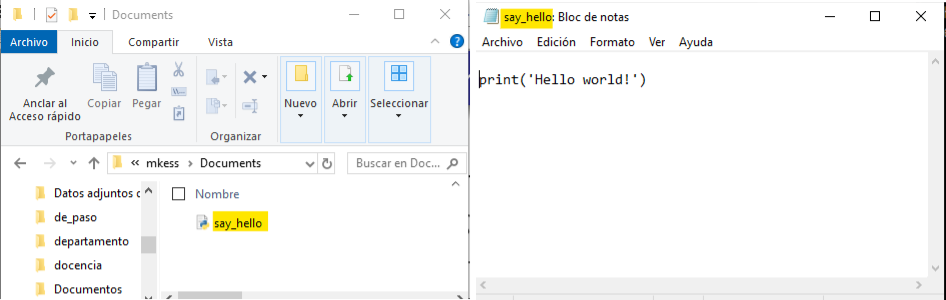
\includegraphics[width=0.9\textwidth]{say_hello_composition}
            \end{center}
            \pause
            Ejecutad el fichero desde la consola Anaconda usando la
            instrucción
            \inlinecode[bash]{python name_file.py}:
            \begin{center}
              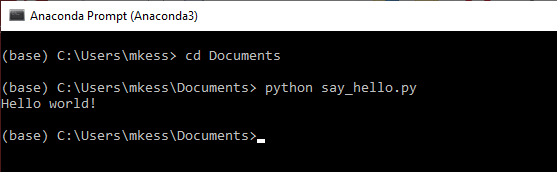
\includegraphics[width=0.9\textwidth]{say_hello_prompt}
            \end{center}
            
          \end{frame}
          \begin{frame}{Usando un bloc de notas Jupyter }
            Los blocs de notas Jupyter permiten elaborar documentos
            que combinan texto formateado (usando 
            \href{https://en.wikipedia.org/wiki/Markdown}{síntaxis
              Markdown}), celdas que contengan código Python y el
            resultado de la ejecución de estas celdas.
            \begin{center}
              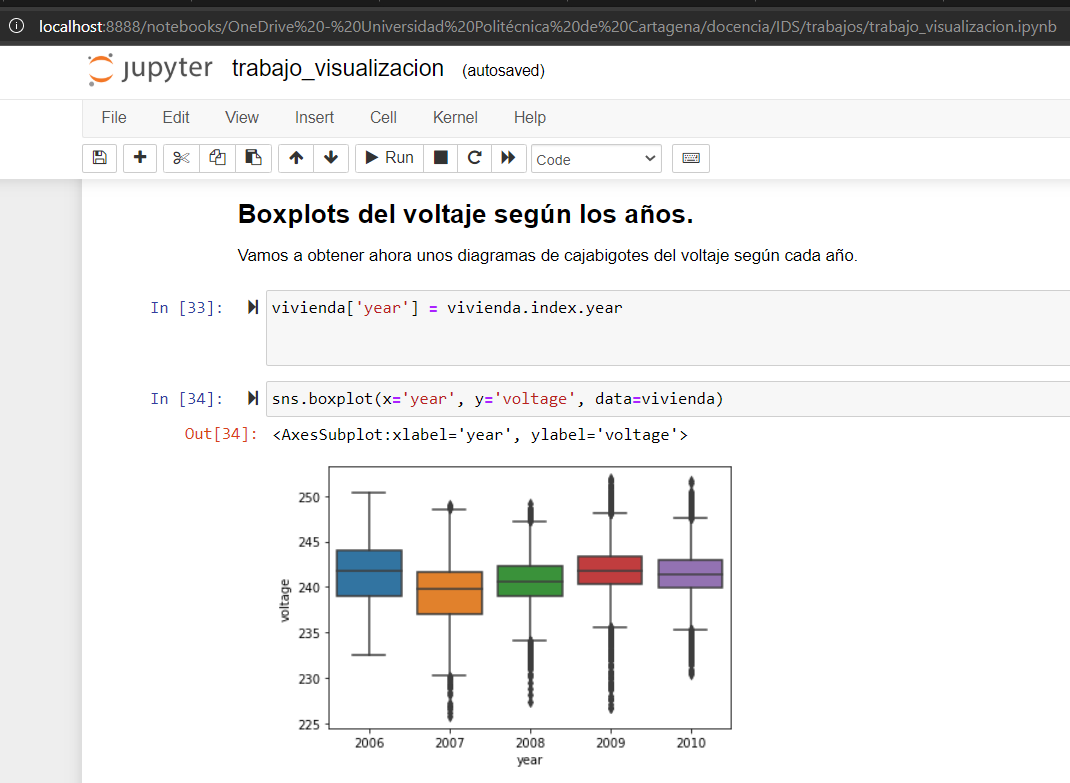
\includegraphics[width=0.9\textwidth]{jupyter_notebook}
            \end{center}
          \end{frame}
          \begin{frame}{Usaremos estos tres métodos desde dentro de  Visual Studio Code}
            \begin{center}
              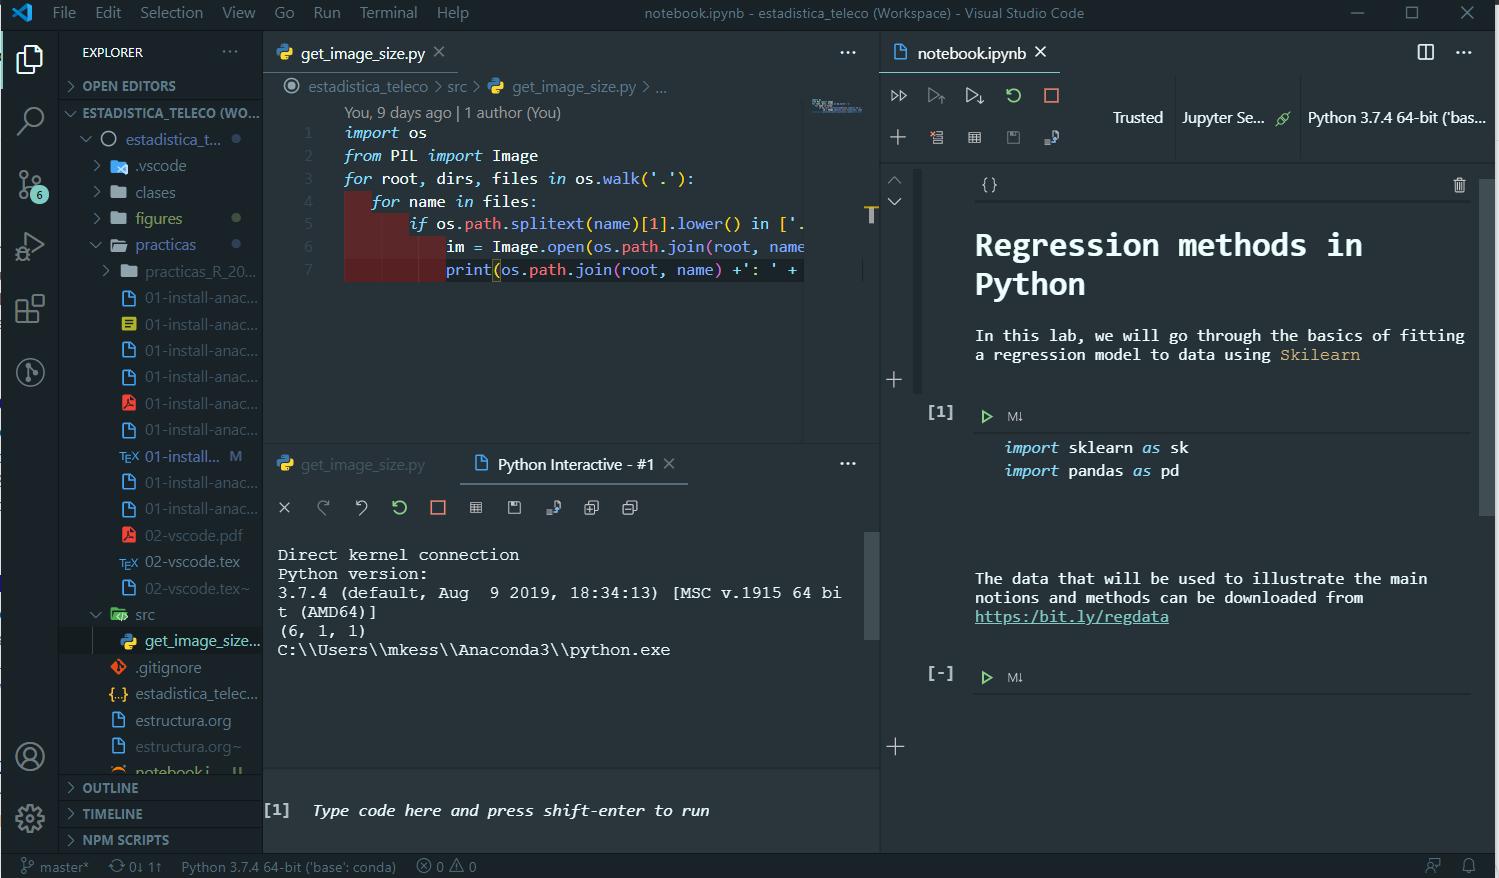
\includegraphics[width=1.05\textwidth]{visual_studio_code_three_methods}
            \end{center}
          \end{frame}
          

        \end{document}
